\documentclass[a4paper]{common/rendering_solutions}
\usepackage[utf8]{inputenc}
\usepackage{epsfig}
\usepackage{amsfonts}
\usepackage{amsmath}
\usepackage{xcolor}
\usepackage[colorlinks]{hyperref}
\usepackage{subcaption}
\usepackage{listings}
% \usepackage[ngerman]{babel}
\SetCGPageDimensions

\lstset{
  frame=single,
  rulecolor=\color[RGB]{239,240,241},
  backgroundcolor=\color[RGB]{252,252,252},
  basicstyle=\ttfamily\color[RGB]{35,38,41},
  keywordstyle=\color[RGB]{61,174,233},
  commentstyle=\color[RGB]{39,174,96},
  stringstyle=\color[RGB]{218,68,83},
  numbers=left,
  numberstyle=\tiny\color[RGB]{175,176,179},
  keepspaces=true,
  showstringspaces=false,
  tabsize=4,
  language=C++,
  breaklines=true,
  breakatwhitespace=true,
  columns=fullflexible
}


\Lecture{Rendering 2026/27}


% sort packages alphabetically please
\usepackage[backend=biber,style=numeric]{biblatex}
\usepackage{float}
\usepackage{graphicx}
\usepackage{listings}
\usepackage{placeins}
\usepackage{svg}
\usepackage{xcolor}
% sort packages alphabetically please

\lstset{
    language=C++,
    basicstyle=\ttfamily\small,
    numbers=left,
    numberstyle=\tiny\color{gray},
    numbersep=8pt,
    keywordstyle=\color{blue},
    commentstyle=\color{gray}\itshape,
    stringstyle=\color{red!70!black},
    breaklines=true,
    breakatwhitespace=false,
    showstringspaces=false,
    frame=single,
    tabsize=4,
    captionpos=b
}

\addbibresource{references.bib}

\Author{Giorgi Gogelashvili, Simon Sutoris, Erik Lahuerta}
\Assignment{5}
\Date{\today}

\begin{document}

\ExerciseHeader

%\Exercise{Importance Sampling: Diffuse BRDF}
%% sections/5_1_importance_sampling_diffuse_brdf.tex
\begin{enumerate}
  \item    
    The PDF of a uniformly sampled disk of radius 1 and centered at the origin is $\frac{1}{\pi}$ when calculated using cartesian coordinates. If calculated using polar coordinates, it must be taken into account the change from $dxdy = r * d\theta dr$. This results in the PDF in polar coordinates being $\frac{r}{\pi}$.
  
  \item
    To generate samples according to the PDF using inversion sampling, we must convert the samples from a uniform distribution into samples from our unit disk. This is achieved by inverting the CDF and using marginal distributions.
    
    First we must compute the marginal distribution from either $r$ or $\theta$. In our case, we compute the marginal probability distribution with respect to $\theta$:
    
    \[p_{\theta}(\theta)=\int_{0}^{1}\frac{r}{\pi}\space dr = \left[\frac{r^{2}}{2}*\frac{1}{\pi} \right]^{1}_{0} =\frac{1}{2\pi}\]
    
    Now we must compute the CDF by taking the integral from $-\infty$ to $\theta$. Since $\theta$ is in the domain $[0,2\pi)$, we take the integral from $0$ to $\theta$.
    
    \[P_{\theta}(\theta)=\int_{0}^{\theta}\frac{1}{2\pi}\space d\theta = \left[\frac{\theta}{2\pi} \right]^{\theta}_{0} =\frac{\theta}{2\pi}\]

    We now do a similar process with $r$ conditioned to $\theta$:

    \[p(r\mid \theta)=\frac{p(r,\theta)}{p(\theta)}=\frac{\frac{r}{\pi}}{\frac{1}{2\pi}}=2r\]
    
    \[P_{r\mid \theta}(r\mid \theta)=\int_{0}^{r}2r\space dr = \left[\frac{2r^{2}}{2} \right]^{r}_{0} =r^{2}\]
    
    Now, drawing $u_{1}, u_{2}$ from a uniform distribution $U$, we need to convert them to our disk using the inverse from our CDF's:

    \[u_{1}=P_{\theta}(\theta)=\frac{\theta}{2\pi}\space; \space \theta=2\pi*u_{1}\]
    \[u_{2}=P_{{r}\mid{\theta}}(r)=r^{2}\space; \space r=\sqrt{u_{2}}\]
    Finally, we need to re-transform our polar coordinates to cartesian ones, and substitute the polar values into our uniform samples. We know the relation is:
    \[x=r\cos(\theta)=\sqrt{u_{2}}\cos(2\pi*u_{1})\] \[y=r\sin(\theta)=\sqrt{u_{2}}\sin(2\pi*u_{1})\]
  \item Code for squareToUniformDisk(Pdf)
    \begin{lstlisting}[language=C++]
Point2f Warp::squareToUniformDisk(const Point2f &sample) {
    return {
        sqrt(sample.x()) * cos(M_PI * 2 * sample.y()),
        sqrt(sample.x()) * sin(M_PI * 2 * sample.y())
    };
}

float Warp::squareToUniformDiskPdf(const Point2f &p) {
    return (p.y() * p.y() + p.x() * p.x()) <= 1 ? 1 / M_PI : 0.0f;
}
\end{lstlisting}
  \item Code for squareToCosineHemisphere(Pdf)
\begin{lstlisting}[language=C++]
  Vector3f Warp::squareToCosineHemisphere(const Point2f &sample) {
    auto disk = Warp::squareToUniformDisk(sample);
    return {
        disk.x(),
        disk.y(),
        std::sqrt(1.0f - sample.x())
    };
}

float Warp::squareToCosineHemispherePdf(const Vector3f &v) {
    if (v.z() < 0.0f) {
        return 0.0f;
    }

    // v.z() = cos(theta_i)
    return v.z() * INV_PI;
}
\end{lstlisting}

\begin{figure}[H]
    \centering
    \begin{minipage}{0.48\textwidth}
        \centering
        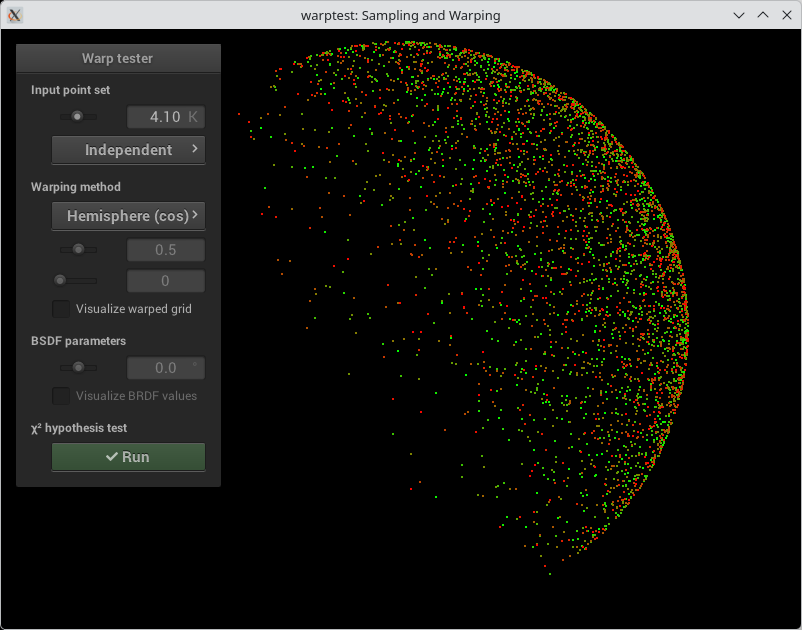
\includegraphics[width=\linewidth]{pictures/warptest-2.png}
        \caption{Transformation of independent samples into the cosine-weighted hemisphere}
        \label{fig:warp-transformation}
    \end{minipage}
    \hfill
    \begin{minipage}{0.48\textwidth}
        \centering
        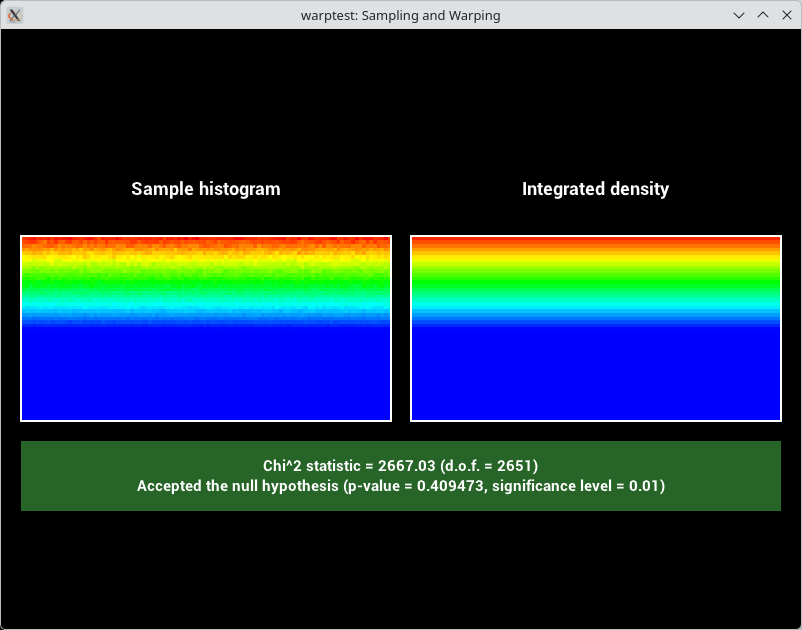
\includegraphics[width=\linewidth]{pictures/warptest-3.png}
        \caption{Successful $X^{2}$ hypothesis test}
        \label{fig:chi-square-test}
    \end{minipage}
\end{figure}
\end{enumerate}

%
%\Exercise{Importance Sampling: BSDF-Aware Path Tracer}
%\subsection{BSDF Path Integrator}

For this exercise, we implement a BSDF path integrator that samples
outgoing directions according to the BSDF instead of uniformly
sampling the hemisphere.

\lstinputlisting[
    language=C++,
    firstline=34,
    lastline=66,
    firstnumber=34,
    caption={BSDF path integrator}
]{../../assignments/integrators/bsdfpath.cpp}

Figure~\ref{fig:bsdf-comparison} compares the results of the
simple path integrator and the BSDF path integrator.

\begin{figure}[htbp]
    \centering
    \begin{minipage}{0.48\textwidth}
        \centering
        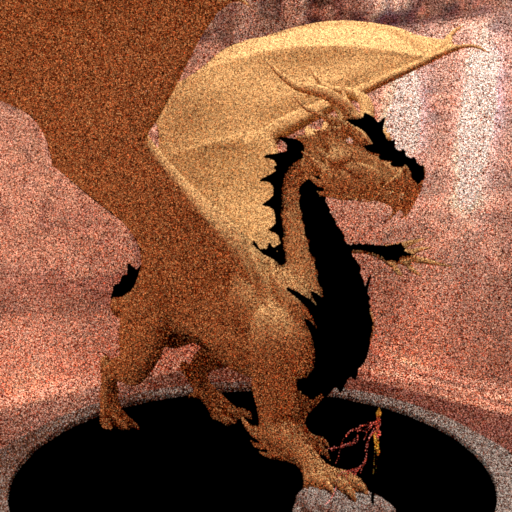
\includegraphics[width=\linewidth]{pictures/dragon-path.png}
        \small (a) Simple path integrator
    \end{minipage}
    \hfill
    \begin{minipage}{0.48\textwidth}
        \centering
        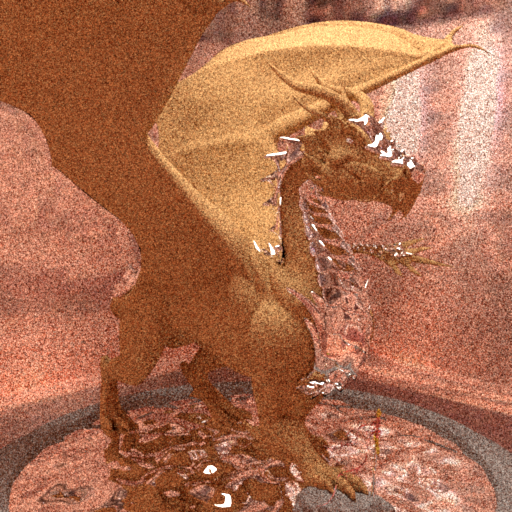
\includegraphics[width=\linewidth]{pictures/dragon-bsdfpath.png}
        \small (b) BSDF path integrator
    \end{minipage}
    \caption{Comparison of uniform hemisphere sampling and BSDF sampling.}
    \label{fig:bsdf-comparison}
\end{figure}

\paragraph{Why do we see this difference?}

With the simple path integrator, we sample directions uniformly over
the hemisphere. For an ideal mirror, the BSDF is nonzero only in the
perfect reflection direction. Since we sample from a continuous
distribution, the probability of choosing this exact direction is zero.

Moreover, the mirror BSDF is a delta distribution, and its
\texttt{eval()} method returns zero even if we somehow happen to sample
the correct direction. As a result, mirror surfaces appear black.

The BSDF path integrator avoids this problem by sampling directions
directly from the BSDF. For mirror surfaces, this means choosing the
reflection direction deterministically and obtaining the corresponding
contribution through \texttt{sample()}, rather than \texttt{eval()}.
%
%\Exercise{Russian Roulette}
%


%scenes/ex05/dragon/dragon-bsdfpath-3-60.xml     24.1s
%scenes/ex05/dragon/dragon-bsdfpath-60-60.xml    48.3s

% set the subsection couter to 3, such that the sections below are rendered as 
% 5.4, 5.5 and 5.6 in case the sections above are commented out.
\setcounter{subsection}{3} 

\Exercise{Theory: Reflection and Refraction}

\paragraph{a) The reflected direction.}

The derivation follows the geometric explanation in
\href{https://www.pbr-book.org/3ed-2018/Reflection_Models/Specular_Reflection_and_Transmission#SpecularReflection}{\textit{Physically Based Rendering}}.

The reflected direction can be computed using simple vector geometry.
The incident direction $\omega_i$, the surface normal $\mathbf{n}$,
and the reflected direction $\omega_r$ all lie in the same plane.
For specular reflection, the reflected direction makes the same
angle with the normal as the incident direction. Therefore,
\[
    \omega_i \cdot \mathbf{n}
    = \omega_r \cdot \mathbf{n}.
\]

We can decompose $\omega_i$ into two components: one parallel
to the surface normal and one perpendicular to it,
\[
    \omega_i = \omega_{\parallel} + \omega_{\perp}.
\]
Since $\mathbf{n}$ is a unit vector,
\[
\begin{aligned}
    \omega_{\parallel}
        &= (\omega_i \cdot \mathbf{n})\mathbf{n},\\
    \omega_{\perp}
        &= \omega_i - (\omega_i \cdot \mathbf{n})\mathbf{n}.
\end{aligned}
\]

For perfect reflection, the normal component stays the same,
while the perpendicular component changes sign. Thus,
\[
\begin{aligned}
    \omega_r
        &= \omega_{\parallel} - \omega_{\perp}\\
        &= \omega_{\parallel} - (\omega_i-\omega_{\parallel})\\
        &= -\omega_i + 2(\omega_i\cdot\mathbf{n})\mathbf{n}.
\end{aligned}
\]

\paragraph{b) The local direction.}

In local coordinates, the surface normal is
$\mathbf{n}=(0,0,1)^\top$. Substituting this into the
reflection equation gives
\[
\begin{aligned}
    \omega_r
        &= -\omega_i + 2(\omega_i\cdot\mathbf{n})\mathbf{n}\\
        &= -(\omega_x,\omega_y,\omega_z)^\top
           + 2\omega_z(0,0,1)^\top\\
        &= (-\omega_x,-\omega_y,\omega_z)^\top.
\end{aligned}
\]


\paragraph{c) The refracted direction.}

Since incident rays can arrive from either side of the surface,
we first determine the incident and transmitted refractive indices:
\[
(\eta_i,\eta_t)=
\begin{cases}
(\eta_{\mathrm{ext}},\eta_{\mathrm{int}}), & \omega_z\geq 0,\\
(\eta_{\mathrm{int}},\eta_{\mathrm{ext}}), & \omega_z<0.
\end{cases}
\]

Let $\eta=\eta_i/\eta_t$. From Snell's law,
\[
    \eta_i\sin\theta_i=\eta_t\sin\theta_t.
\]
Like in reflection all vectors lie in the same plane.
For unit directions, the sine of the angle with the normal
equals the length of the perpendicular component. Therefore,
\[
    \omega_{t,x}=-\eta\omega_x,\qquad
    \omega_{t,y}=-\eta\omega_y.
\]

Since $\omega_t$ must also be a unit vector,
\[
    \omega_{t,z}^2=1-\eta^2(1-\omega_z^2).
\]
If we assume that the refracted direction points into the opposite medium,
its normal component has the opposite sign to $\omega_z$:
\[
\omega_t=
\begin{pmatrix}
-\eta\omega_x\\
-\eta\omega_y\\
-\operatorname{sgn}(\omega_z)
\sqrt{1-\eta^2(1-\omega_z^2)}
\end{pmatrix}.
\]


\Exercise{Conductor and Dialectric BSDF}
\begin{enumerate}
\item % (a)

Our implementation for the Fresnel term is found in Listing \ref{lst:5-5-a}.

\begin{lstlisting}[caption={Function to compute the Fresnel term},label={lst:5-5-a}]
float compute_fresnel(const Vector3f& v, float eta, float k) {
    float sin = Frame::sinTheta(v);
    float cos = Frame::cosTheta(v);
    float tan = Frame::tanTheta(v);
    float sin2 = sin * sin;
    float cos2 = cos * cos;
    float tan2 = tan * tan;

    float eta2 = eta * eta;
    float k2 = k * k;
    float eta2k2sin2 = eta2 - k2 - sin2;

    float root = std::sqrt(eta2k2sin2 * eta2k2sin2 + 4 * eta2 * k2);
    float a2 = 0.5 * (root + eta2k2sin2);
    float b2 = 0.5 * (root - eta2k2sin2);
    float a = std::sqrt(a2);

    float R_s = (a2 + b2 - 2 * a * cos + cos2) /
                (a2 + b2 + 2 * a * cos + cos2);

    float R_p = R_s * (a2 + b2 - 2 * a * sin * tan + sin2 * tan2) /
                      (a2 + b2 + 2 * a * sin * tan + sin2 * tan2);

    return 0.5f * (R_s + R_p);
}
\end{lstlisting}

\item % (b)

Our implementation for the conductor BSDF model is found in Listing \ref{lst:5-5-b}.

\begin{lstlisting}[caption={Our implementation for the conductor BSDF model},label={lst:5-5-b}]
#include "nori/common.h"
#include <cmath>
#include <cstdlib>
#include <nori/bsdf.h>
#include <nori/texture.h>
#include <nori/frame.h>
#include <nori/warp.h>

NORI_NAMESPACE_BEGIN

/**
 * \brief Conductor BRDF model
 */
class Conductor : public BSDF {
public:
    Conductor(const PropertyList &propList) {
        m_eta = propList.getColor("eta");
        m_k = propList.getColor("k");
    }

    /**
     * \brief Evaluate the BSDF for a pair of directions and measure
     * specified in \code bRec
     *
     * \param bRec
     *     A record with detailed information on the BSDF query
     * \return
     *     The BSDF value, evaluated for each color channel
     */
    Color3f eval(const BSDFQueryRecord &bRec) const override {
        return {0.0f};
    }

    /**
     * \brief Compute the probability of sampling \c bRec.wo
     * (conditioned on \c bRec.wi).
     *
     * This method provides access to the probability density that
     * is realized by the \ref sample() method.
     *
     * \param bRec
     *     A record with detailed information on the BSDF query
     *
     * \return
     *     A probability density value expressed with respect
     *     to the specified measure
     */
    float pdf(const BSDFQueryRecord &bRec) const override {
        return 0.0f;
    }

    /**
     * \brief Sample the BSDF and return the importance weight (i.e. the
     * value of the BSDF * cos(theta_o) divided by the probability density
     * of the sample with respect to solid angles).
     *
     * \param bRec    A BSDF query record
     * \param sample  A uniformly distributed sample on \f$[0,1]^2\f$
     *
     * \return The BSDF value divided by the probability density of the sample,
     *         multiplied by the cosine factor associated with the outgoing direction.
     *         A zero value means that sampling failed.
     */
    Color3f sample(BSDFQueryRecord &bRec, const Point2f &sample) const override {
        bRec.wo = Vector3f{
            -bRec.wi.x(),
            -bRec.wi.y(),
            bRec.wi.z(),
        };

        Color3f F_r(
            compute_fresnel(bRec.wo, m_eta.r(), m_k.r()),
            compute_fresnel(bRec.wo, m_eta.g(), m_k.g()),
            compute_fresnel(bRec.wo, m_eta.b(), m_k.b())
        );
        bRec.measure = EDiscrete;

        float costheta = std::abs(Frame::cosTheta(bRec.wo));
        return {
            F_r.r() / costheta,
            F_r.g() / costheta,
            F_r.b() / costheta,
        };
    }

    /// Return a human-readable summary
    std::string toString() const override {
        return tfm::format(
                    "Conductor[\n"
                    "  eta = %s,\n"
                    "  k = %s,\n"
                    "]", m_eta.toString(), m_k.toString());
    }

    EClassType getClassType() const  override { return EBSDF; }
private:
    Color3f m_eta;
    Color3f m_k;
};

NORI_REGISTER_CLASS(Conductor, "conductor");
NORI_NAMESPACE_END

\end{lstlisting}

\item % (c)

Our implementation for the dielectric BSDF model is found in Listing \ref{lst:5-5-c}.

\begin{lstlisting}[caption={Our implementation for the dielectric BSDF model},label={lst:5-5-c}]
#include <nori/bsdf.h>
#include <nori/texture.h>
#include <nori/frame.h>
#include <nori/warp.h>

NORI_NAMESPACE_BEGIN

/**
 * \brief Dielectric BRDF model
 */
class Dielectric : public BSDF {
public:
    Dielectric(const PropertyList &propList) {
        m_extIOR = propList.getFloat("extIOR");
        m_intIOR = propList.getFloat("intIOR");
    }

    /**
     * \brief Evaluate the BSDF for a pair of directions and measure
     * specified in \code bRec
     *
     * \param bRec
     *     A record with detailed information on the BSDF query
     * \return
     *     The BSDF value, evaluated for each color channel
     */
    Color3f eval(const BSDFQueryRecord &bRec) const override {
        return {0.0f};
    }

    /**
     * \brief Compute the probability of sampling \c bRec.wo
     * (conditioned on \c bRec.wi).
     *
     * This method provides access to the probability density that
     * is realized by the \ref sample() method.
     *
     * \param bRec
     *     A record with detailed information on the BSDF query
     *
     * \return
     *     A probability density value expressed with respect
     *     to the specified measure
     */
    float pdf(const BSDFQueryRecord &bRec) const override {
        return 0.0f;
    }

    /**
     * \brief Sample the BSDF and return the importance weight (i.e. the
     * value of the BSDF * cos(theta_o) divided by the probability density
     * of the sample with respect to solid angles).
     *
     * \param bRec    A BSDF query record
     * \param sample  A uniformly distributed sample on \f$[0,1]^2\f$
     *
     * \return The BSDF value divided by the probability density of the sample,
     *         multiplied by the cosine factor associated with the outgoing direction.
     *         A zero value means that sampling failed.
     */
    Color3f sample(BSDFQueryRecord &bRec, const Point2f &sample) const override {
        bRec.wi.normalize();
        bRec.measure = EDiscrete;

        // determine the incident and transmitted IOR
        float etaI = m_extIOR;
        float etaT = m_intIOR;
        float sgn = 1.0;

        if (bRec.wi.z() < 0.0f) {
            std::swap(etaI, etaT);
            sgn = -1.0;
        }

        // relative IOR
        float eta = etaI / etaT;

        // fresnel reflectance
        float cosThetaI = std::abs(bRec.wi.z());
        float F_r = fresnelDielectric(cosThetaI, etaI, etaT);

        // reflection direction
        Vector3f wr = Vector3f{
            -bRec.wi.x(),
            -bRec.wi.y(),
            bRec.wi.z(),
        };

        // check for total internal reflection
        float sinThetaT2 = eta * eta * (1.0f - cosThetaI * cosThetaI);

        if (sinThetaT2 >= 1.0) {
            bRec.wo = wr;
            return {1.0f};
        }

        // choose relfection or refraction
        if (F_r > sample.x()) {
            // reflection
            bRec.wo = wr;
            return {1.0};
        } else {
            // refraction
            float cosThetaT = std::sqrt(1.0f - sinThetaT2);

            bRec.wo = Vector3f{
                -eta * bRec.wi.x(),
                -eta * bRec.wi.y(),
                -sgn * cosThetaT,
            };

            bRec.eta = etaT / etaI;
            return {eta * eta};
        }
    }

    /// Return a human-readable summary
    std::string toString() const override {
        return tfm::format(
                    "Dielectric[\n"
                    "  extIOR = %f,\n"
                    "  intIOR = %f,\n"
                    "]", m_extIOR, m_intIOR);
    }

    EClassType getClassType() const  override { return EBSDF; }

    void computeReflectance(float n, float k, float& R_s, float& R_p) {
    }
private:
    float m_extIOR;
    float m_intIOR;
};

NORI_REGISTER_CLASS(Dielectric, "dielectric");
NORI_NAMESPACE_END

\end{lstlisting}

\item % (d)

Our code for the conductor does not seem correct. It is way too bright in comparison to the reference image. Especially close surfaces, which are parallel to each other, appear to generate light. This is seen in the comparison Figure \ref{fig:ingots-compare}, which has a green tint. This probably results from the values of each pixel or our result being significantly higher than the reference. We couldn't fiure out the correct code and decided to turn it in anyway.

The dialectric translucent ingot appears correct however. The parts of it that are not bent into a conducting ingot are quite dark in the comparison, suggesting that the returned color is correct.

\begin{figure}[H]
    \centering
    \begin{minipage}{0.32\textwidth}
        \centering
        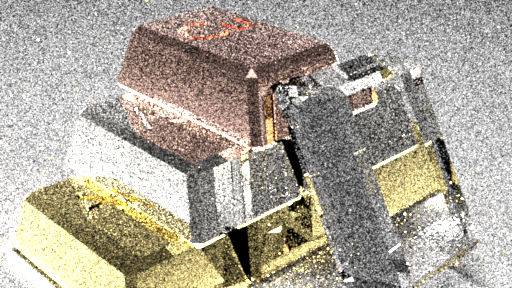
\includegraphics[width=\linewidth]{pictures/ingots-bsdfpath.png}
        \caption{Our result of the ingots scene}
        \label{fig:ingots-result}
    \end{minipage}
    \hfill
    \begin{minipage}{0.32\textwidth}
        \centering
        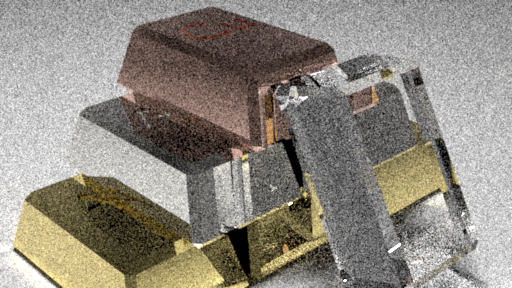
\includegraphics[width=\linewidth]{pictures/ingots-bsdfpath-512spp-ref.png}
        \caption{The reference image of the ingots scene}
        \label{fig:ingots-reference}
    \end{minipage}
    \hfill
    \begin{minipage}{0.32\textwidth}
        \centering
        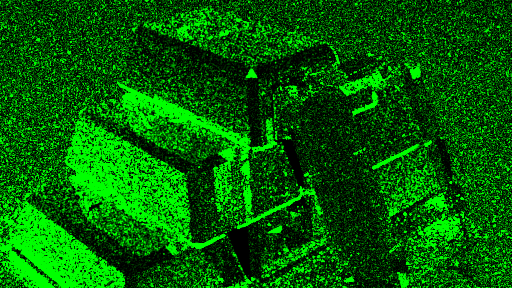
\includegraphics[width=\linewidth]{pictures/ingots-bsdfpath-compare.png}
        \caption{Comparison between our result vs reference}
        \label{fig:ingots-compare}
    \end{minipage}
\end{figure}

\end{enumerate}

\Exercise{Bonus: Step-by-Step Derivation of Hemisphere Sampling}
\documentclass{article}
\usepackage{graphicx} % Required for inserting images
\usepackage{amsmath}

\title{Ex 5.5}
\author{ERIK LAHUERTA ARTIEDA}
\date{November 2026}

\begin{document}

\maketitle

\subsection{Preliminaries \& Notation}
We will be drawing our uniform samples from a uniform distribution $U(0,1) \sim r_{1}, r_{2}$.\newline \newline
$w$ is our vector representation on the sphere, given by the convention $(r,\theta, \varphi)$, where r is the radius, $\theta$ is the polar angle, and $\varphi$ is the azimuthal angle. Since we are only interested in directions, r is not relevant. Then our differentials follow:
\[dw = sin(\theta)\space d\theta d\varphi\]
Similarly, because we are interested in $p(w)$, but want to convert to our angles, it also follows that:
\[p(w)=p(\theta, \varphi)\space sin(\theta)\] \newline
On cartesian coordinates, the conversion from polar to cartesian is as follows:
\[x=r\sin(\theta)\cos(\varphi)\]
\[y=r\sin(\theta)\sin(\varphi)\]
\[z=r\cos(\theta)
\]
These properties are used throughout the rest of the exercise and are useful to keep in mind.

\subsection{Uniformly Sampling a Hemisphere}
We will use inversion sampling. Sampling uniformly across the hemisphere means that: $p(w)=c$ for all $w$. Because this is a density function, it must mean that the integral over the domain must be equal to 1. Then:
\begin{align*}
\int_{H^{2}}p(w) dw
&=\int_{0}^{2\pi}\int_{0}^{2/\pi}c\ sin(\theta)\ d\theta d\varphi \\
&= c\int_{0}^{2\pi}\int_{0}^{2/\pi}sin(\theta) \ d\theta d\varphi \\
&= c\int_{0}^{2\pi}\left[-\cos(\theta)\right]^{2/\pi}_{0} d\varphi \\
&= c\int_{0}^{2\pi}1\ d\varphi \\
&=c*2\pi=1; \\ 
p(w) &=\frac{1}{2\pi}\ ;\\
p(\theta, \varphi) &= \frac{sin(\theta)}{2\pi} 
\end{align*}

Now that we have the joint distribution, we must find the marginal and conditional distributions. In this case, we will condition $\varphi\vert\theta$, although the reverse is valid as well.

\[
p_{\theta}(\theta)=\int^{2\pi}_{0}p(\theta, \varphi)\ d\varphi = \int^{2\pi}_{0}\frac{\sin(\theta)}{2\pi}\ d\varphi=\left[\varphi\frac{\sin(\theta)}{2\pi} \right]^{2\pi}_{0} = \sin(\theta)
\]
\[
p_{\varphi\vert\theta}(\varphi\vert\theta)=\frac{p(\theta,\varphi)}{p(\theta)}=\frac{\frac{\sin(\theta)}{2\pi}}{\sin(\theta)}=\frac{1}{2\pi}
\]

Now that we have found the marginal and conditional densities, we must find their CDF's in order to apply the inversion method:

\[
P_{\theta}(\theta)=\int_{0}^{\theta} \sin(\theta)\ d\theta= 1-\cos(\theta)
\]
\[
P_{\varphi\vert\theta}(\varphi\vert\theta) = \int^{\varphi}_{0}\frac{1}{2\pi}\ d\varphi = \frac{\varphi}{2\pi}
\]
Now we must apply the inversion method in order to convert uniform variables from 0 to 1 into uniformly distributed samples in polar coordinates.
\[
P_{\theta}(\theta)=1-\cos(\theta)=r_{1};\ \theta=\cos^{-1}(1-r_{1})=\cos^{-1}(r_{1})
\]
\[
P_{\varphi\vert\theta}(\varphi\vert\theta)=\frac{\varphi}{2\pi}=r_{2};\ \varphi =2\pi r_{2}
\]
We can safely convert $1-r_{1}$ to $r_{1}$, since both uniformly go from 0 to 1, but reversed.
We now have a conversion from uniform variables into our polar angles. The last step is to convert from polar coordinates to cartesian coordinates. Since we are only sampling the direction, a simplifying step is saying that the radius is 1.
There are useful trigonometric properties for the sake of simplification. One of them is: $\sin(\cos^{-1}(x))=\sqrt{1-x^{2}}$. Then it follows that: $\sin(\theta)=\sqrt{1-r_{1}^{2}}$
Another useful property is $\cos(\cos^{-1}(x))=x. $ It then follows that: $\cos(\theta)=r_{1}$
\begin{align*} 
x&=\sqrt{1-r_{1}^{2}}\ *\cos(2\pi r_{2}) \\
y&=\sqrt{1-r_{1}^{2}}\ *\sin(2\pi r_{2}) \\
z&=r_{1}
\end{align*}
This is the final result that we need to implement the sampling.
\subsection{Cosine-Weighted Hemisphere Sampling}
This time, we would like to sample from a PDF $p(w)\propto\cos(\theta)$. Following the process from last section:
\begin{align*}
\int_{H^{2}}p(w)\  dw
&=\int_{0}^{2\pi}\int_{0}^{2/\pi}c\ \cos(\theta)\sin(\theta)\ d\theta d\varphi \\
&= c\int_{0}^{2\pi}\left[-\frac{1}{2}\cos^{2}(\theta)\right]^{2/\pi}_{0} d\varphi \\
&= c\int_{0}^{2\pi}0.5\ d\varphi \\
&=c*\pi=1; \\ 
p(w) &=\frac{1}{\pi}\ ;\\
p(\theta, \varphi) &= \frac{\cos(\theta)\sin(\theta)}{\pi} 
\end{align*}
Instead of computing marginal and conditional densities, this time we shall use \textit{Malley's method} to generate the cosine-weighted points. This method consists of generating uniform samples on the unit disk, projecting them to the hemisphere above, and computing the direction from the center of the sphere. 
Using this method, we can use the sampling that was used on the disk sampling: $(r,\theta)=(\sqrt{r_{1}}, 2\pi r_{2})$. This method is equivalent to the points that we would obtain from doing the inversion method, so the final samples end up being the same.
\end{document}


%===============================================================================
% References
%===============================================================================
\FloatBarrier
\printbibliography

\end{document}

